\documentclass{beamer}
%%%%%%%%%%%%%%%%%%%%%%
% basic tutorial in german: http://www2.informatik.hu-berlin.de/~mischulz/beamer.html
%%%%%%%%%%%%%%%%%%%%%%

%------- packages ---------%
\usepackage[english]{babel}         %Umlaute, neue deutsche Rechtschreibung
\usepackage[utf8x]{inputenc}        %Kodierung festlegen, für UTF-8 Unterstützung entsprechend 
\usepackage{amsmath,amsfonts,amssymb}   %math. Symbole und Umgebungen
\usepackage{graphicx}
\usepackage{array}
\newcolumntype{P}[1]{>{\raggedright\arraybackslash}p{#1}}
\usepackage{color} % use color

%\usepackage{natbib}
%------- theme and style ---------%
\usetheme{Boadilla}  %% Themenwahl
\usecolortheme{default}
\usefonttheme{default}
\useinnertheme{circles}     %	{circles | default | inmargin |	rectangles | rounded}
\useoutertheme{default} %	default | infolines | miniframes | shadow | sidebar | smoothbars |smoothtree | split | tree}
\bibliographystyle{apalike}
%\beamertemplatenavigationsymbolsempty   % disable navigation simbols
%\bibliographystyle{apalike}
%------- metainformation ---------%

\title[Elementary mode analysis]{Designing optimal cell factories:
integer programming couples elementary mode analysis with regulation\\~\\}
\subtitle{Molecular Networks B SS13}
\author[Jonas Ibn-Salem]{Jonas Ibn-Salem}
\institute[]{}
\date{25.04.13}
%\logo{\pgfimage[width=2cm,height=0.5cm]{grafik/FULogo_RGB}}
\titlegraphic{
\includegraphics[width=4cm,height=1cm]{grafik/FULogo_RGB}}


\begin{document}
%\frame{\titlepage}
\maketitle

% OUTLINE:
%- Metabolically engineering: 
%  - strain improvement 
%  - efficient deletion strategies
% -steady state assumption, 
% -elementary mode (EM)
% -constrained minimal cut sets
% -network of minimal functionality
% -advantage of inclusion of regulatory information
%%%%%%%%%%%%%%%%%%%%%%%%%%%%%%%%%%%%%%%%%%%%%%%%%%%%%%%%%%%%%%%%%%%%%%%% 
% Preface stuff:
%%%%%%%%%%%%%%%%%%%%%%%%%%%%%%%%%%%%%%%%%%%%%%%%%%%%%%%%%%%%%%%%%%%%%%%% 

\begin{frame}{Overview}
    \tableofcontents
\end{frame}

%%%%%%%%%%%%%%%%%%%%%%%%%%%%%%%%%%%%%%%%%%%%%%%%%%%%%%%%%%%%%%%%%%%%%%%% 
\section{Introduction and Repetition}
%%%%%%%%%%%%%%%%%%%%%%%%%%%%%%%%%%%%%%%%%%%%%%%%%%%%%%%%%%%%%%%%%%%%%%%% 
\subsection{Metabolic network in steady state}
%%%%%%%%%%%%%%%%%%%%%%%%%%%%%%%%%%%%%%%%%%%%%%%%%%%%%%%%%%%%%%%%%%%%%%%% 
\begin{frame}{Metabolic network}
    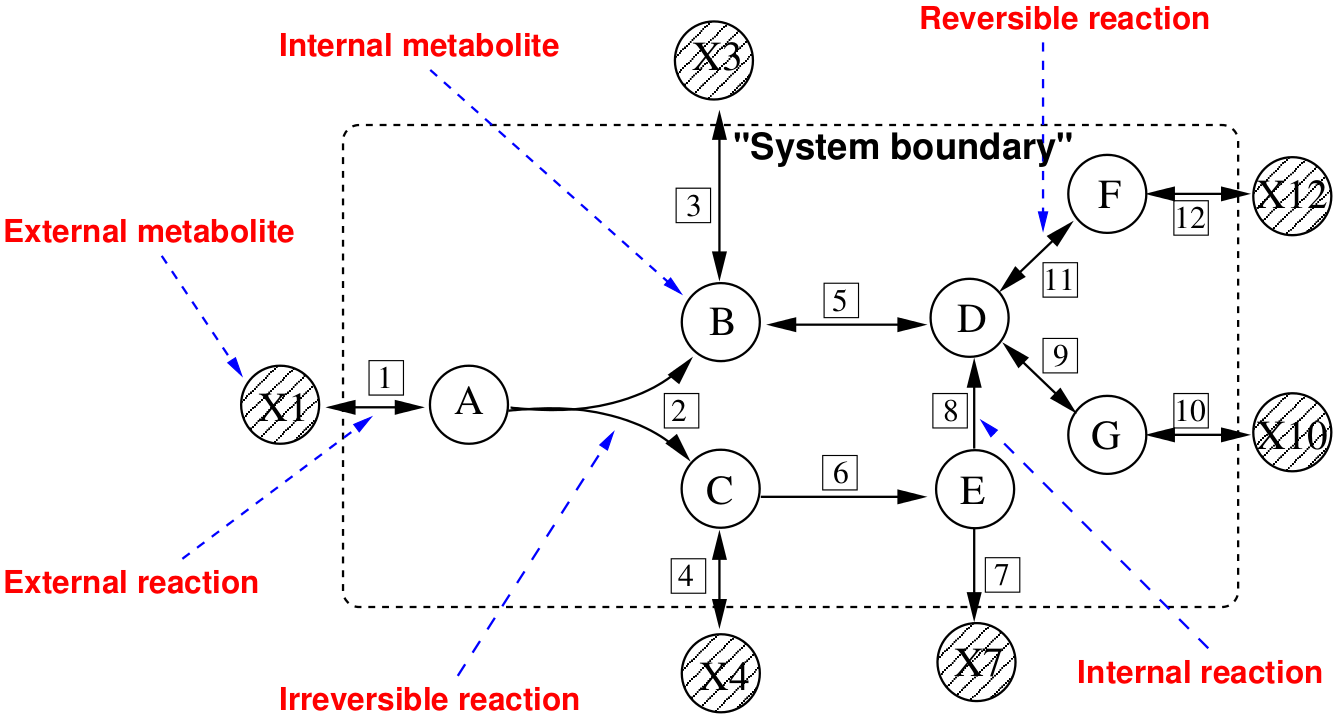
\includegraphics[width=\textwidth]{grafik/molnet}
\end{frame}

\begin{frame}{Metabolic network: Kinetic modelling}
	Model of metabolic network:
\begin{columns}
    \column{0.7\textwidth}
	\begin{itemize}
		\item Internal metabolites $i = 1, ..., m$ 
		\item Reactions $j = 1, ..., n$
		\item Stoichiometric matrix $S \in \mathbb{R}^{m\times n}$
		\item Set of irreversible reactions $Irr \subseteq \{1, ..., n\}$
		\item Flux vector $v \in \mathbb{R}^{n}$, $v_j$ flux through reaction $j$
	\end{itemize}
    \pause
    \column{0.3\textwidth}
    $$\frac{dC_{i}}{dt} = \sum_{j=1}^{n} S_{ij} v_{j} $$
    $$\frac{dC}{dt} = S \cdot v$$
\end{columns}

\end{frame}
\begin{frame}{Metabolic network: Stoichiometric modelling}
%\begin{frame}{Steady state assumption}    
    \begin{block}{Steady state assumption}
        Metabolite concentrations and reaction rates are constant.
    \end{block}
    \begin{itemize}
        \item Mass balance: Rate of production = Rate of consumption
        \item \textcolor{blue}{Steady state flux coen}:
    $$C = \{v \in \mathbb{R}^n | Sv = 0, v_i \geq 0, i \in Irr \}$$
    \end{itemize}
    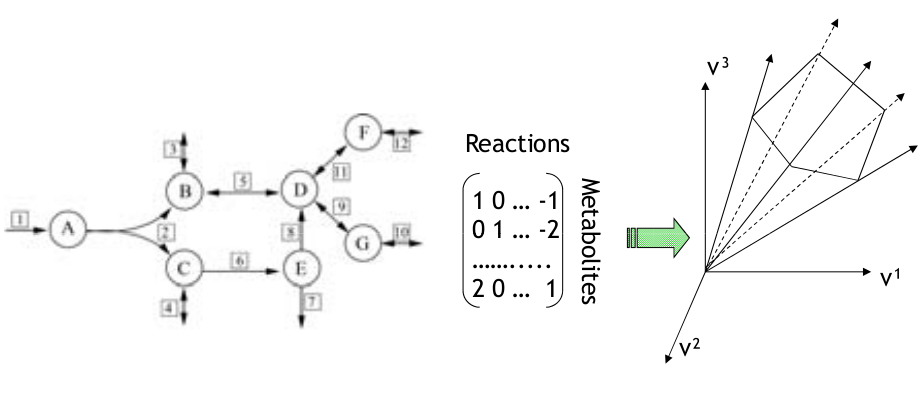
\includegraphics[width=\textwidth]{grafik/modelling} \\
    \hfill \tiny{source A.Bockmayer lecture slides Algorithms in Systembiology SS12}
\end{frame}

%%%%%%%%%%%%%%%%%%%%%%%%%%%%%%%%%%%%%%%%%%%%%%%%%%%%%%%%%%%%%%%%%%%%%%%% 
\subsection{Elementary flux modes}

\begin{frame}{Elementary flux modes (EM)}
    \begin{itemize}
        %\item Steady state flux coen 
        %$C = \{v \in \mathbb{R}^n | Sv = 0, v_i \geq 0, i \in Irr \}$
        \item For $v \in \mathbb{R}^n$, the \textcolor{blue}{support}
         of $v$ is defined as 
        $supp(v) = \{i \in \{1, ..., n \} | v_i \neq 0  \}$
        
        \item $v \in C$ is an \emph{\textcolor{blue}{elementary flux mode}} if $supp(v)$
        is minimal w.r.t $\subseteq$
        i.e., if there is no $v' \in C, v' \neq 0$ with 
        $supp(v') \underset{\neq}{\subset} supp(v)$. % \subsetneq
\pause
        \item Any $v \in C$ can be written as a non-negative linear 
        combination of elementary flux modes $e_{1}, ... e_{q}$
        $$v = \lambda_{1} e_{1} + ... + \lambda_{q} e_{q} 
        \quad\quad \lambda_{1}, ..., \lambda{q} \geq 0 $$ %\in \mathbb{R} $$
    \end{itemize}    
\pause
    \begin{block}{}
        An elementary mode (EM) is a minimal and indivisible set 
        of reactions that operates under steady state conditions, 
        while obeying all (ir-)reversibility constraints.
    \end{block}
    
    \begin{itemize}
    	\item Elementary modes correspond to minimal biological pathways.
    \end{itemize}
    
\end{frame}
\begin{frame}{Elementary mode example}
    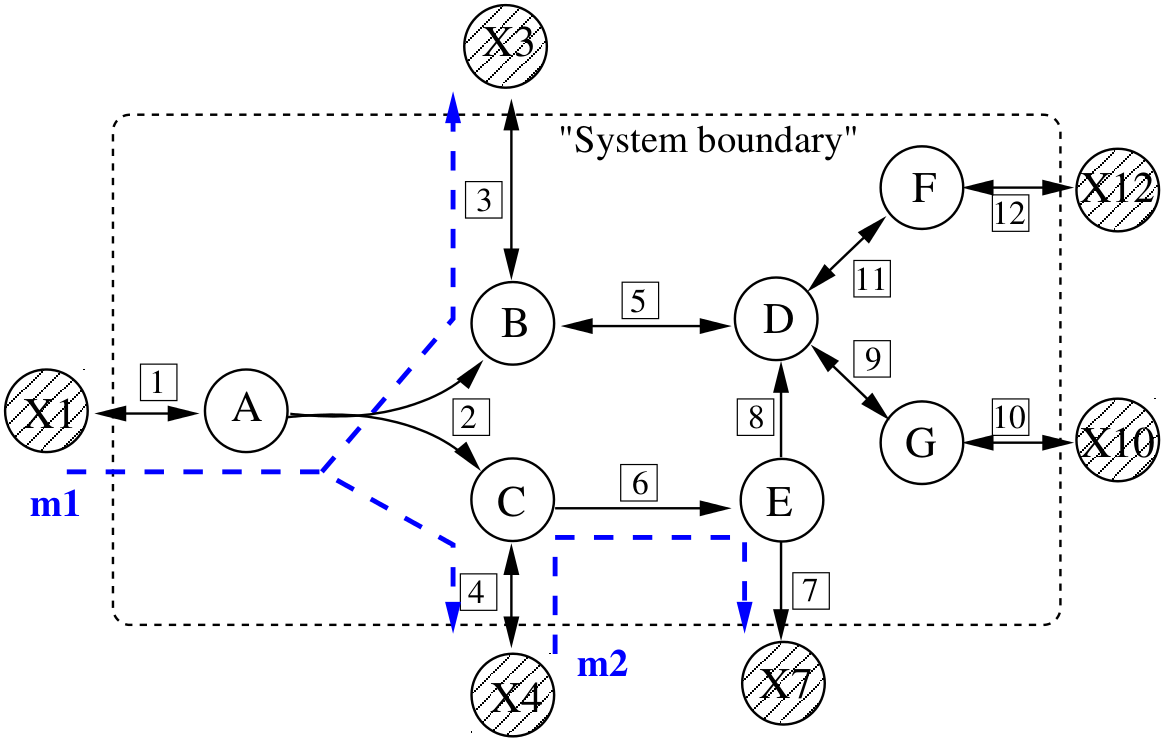
\includegraphics[width=.65\textwidth]{grafik/EMnet1}
    \\
    \hfill \tiny{source: A.Bockmayr lecture slides "Algorithms in Systembiology" SS12}
    \normalsize
    \begin{itemize}
        \item $m^{1} = (1, 1, 1, 1, 0, 0, 0, 0, 0, 0, 0 ,0)$
        \item $m^{1} = (0, 0, 0, -1, 0, 1, 1, 0, 0, 0, 0 ,0)$
\pause
        \item $m^{1}$ and $m^{2}$ are elementary modes.
    \end{itemize}
\end{frame}

\begin{frame}{Elementary mode example (ctd)}
    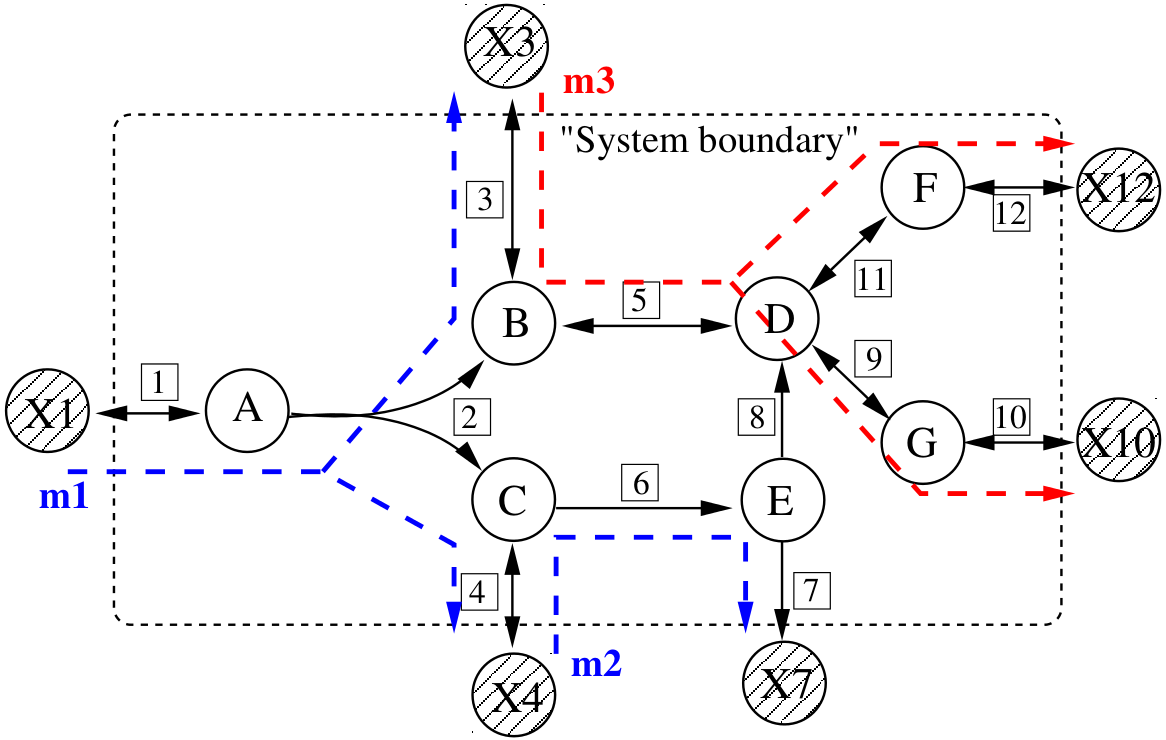
\includegraphics[width=.65\textwidth]{grafik/EMnet2}
    \\
    \hfill \tiny{source: A.Bockmayr lecture slides "Algorithms in Systembiology" SS12}
    \normalsize
    \begin{itemize}
        \item $m^{3} = (0, 0, 2, 0, 2, 0, 0, 0, 1, 1, 1 ,1)$
\pause
        \item $m^{3} = m^{4} + m^{5}$, with
        \begin{itemize}
            \item $ m^{4} = (0, 0, 1, 0, 1, 0, 0, 0, 1, 1, 0 ,0)$
            \item $ m^{5} = (0, 0, 1, 0, 1, 0, 0, 0, 0, 0, 1 ,1)$
        \end{itemize}
        \item Since $m^{4}, m^{5} \in C, supp(m^{4}), supp(m^{5}) \subsetneq supp(m^{3})$, 
        $m^{3}$ is not an elementary flux mode.
    \end{itemize}
\end{frame}

%%%%%%%%%%%%%%%%%%%%%%%%%%%%%%%%%%%%%%%%%%%%%%%%%%%%%%%%%%%%%%%%%%%%%%%% 
\section{Binary linear programming for a minimal deletion strategy}
%%%%%%%%%%%%%%%%%%%%%%%%%%%%%%%%%%%%%%%%%%%%%%%%%%%%%%%%%%%%%%%%%%%%%%%% 
\subsection{Motivation}
%%%%%%%%%%%%%%%%%%%%%%%%%%%%%%%%%%%%%%%%%%%%%%%%%%%%%%%%%%%%%%%%%%%%%%%% 

\begin{frame}{Paper}
    
\includegraphics[width=1\textwidth]{grafik/paper}
    \begin{columns}
    \column{.3\textwidth}
      \begin{center}
        \begin{figure}
         
\includegraphics[width=0.5\textwidth]{grafik/jungreuthmayer} \\
         \tiny{source: biotec.boku.ac.at}
        \end{figure}
      \end{center}
    \column{.3\textwidth}
      \begin{center}
        \begin{figure}
         
\includegraphics[width=0.5\textwidth]{grafik/zanghellini} \\
         \tiny{source: biotec.boku.ac.at}
        \end{figure}
      \end{center}
    \column{.3\textwidth}
    \tiny {$^{1}$ Austrian Centre of Industrial 
        Biotechnology, Vienna, Austria} 
    \\ ~ \\
    \tiny {$^{2}$ Department of Biotechnology, 
        University of Natural Resources and Life Sciences, 
        Vienna, Austria} 
 \end{columns}
\end{frame}

\begin{frame}{Background and motivation}
    \begin{itemize}
        \item Microbes can be used for metabolic engineering 
        e.g. ethanol production in \emph{E. coli}
        \item Metabolic networks are available for some model organisms
    	\item Design a \emph{\textcolor{blue}{network of minimal functionality (NMF)}}
         by iteratively deleting elementary modes / pathways 
	\end{itemize}
    
    \begin{block}{Goal}
        Gene deletion strategy to optimize the production 
        efficiency of strains.
    \end{block}

    \begin{definition}
        A \emph{\textcolor{blue}{minimal cut set (MCS)}} is a mimial set of deletions, 
        which block undesirable network functionality, like unwanted by-products
    \end{definition}

\end{frame}


%\begin{frame}{Network of minimal functionality (NMF)}    
%\end{frame}
%%%%%%%%%%%%%%%%%%%%%%%%%%%%%%%%%%%%%%%%%%%%%%%%%%%%%%%%%%%%%%%%%%%%%%%%
\subsection{Illustrative example}

\begin{frame}{Illustrative example}
    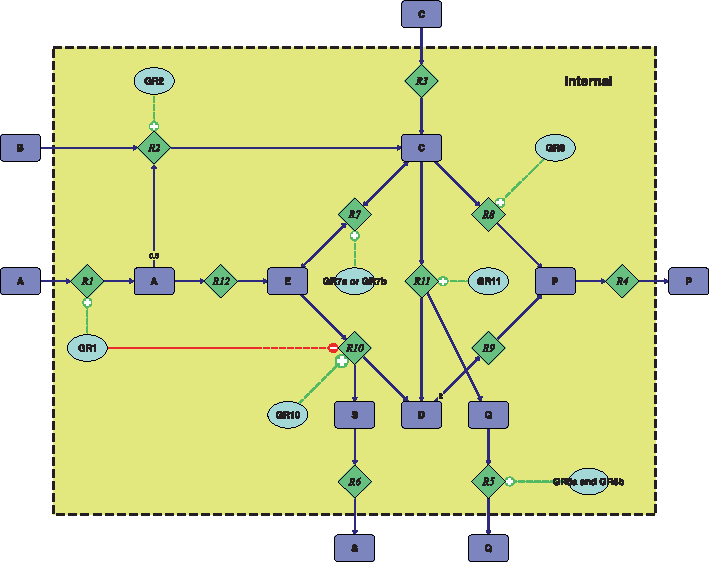
\includegraphics[width=.9\textwidth]{grafik/fig1} \\
\end{frame}

\begin{frame}{Elementary modes}
    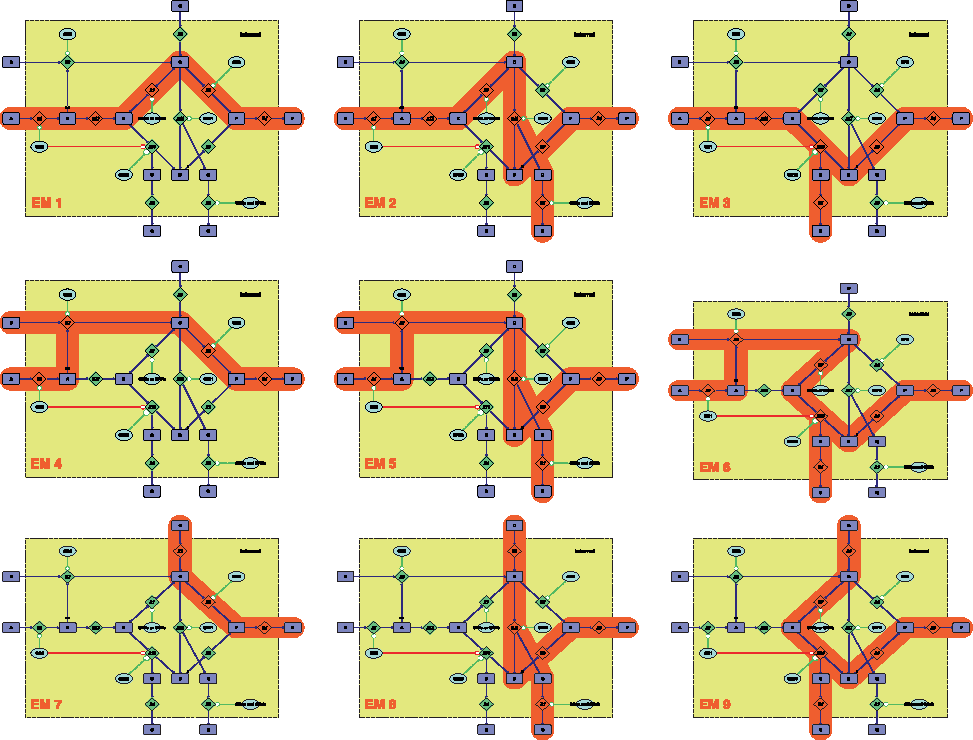
\includegraphics[width=.9\textwidth]{grafik/fig2} \\
\end{frame}

\begin{frame}{List of elementary modes}
    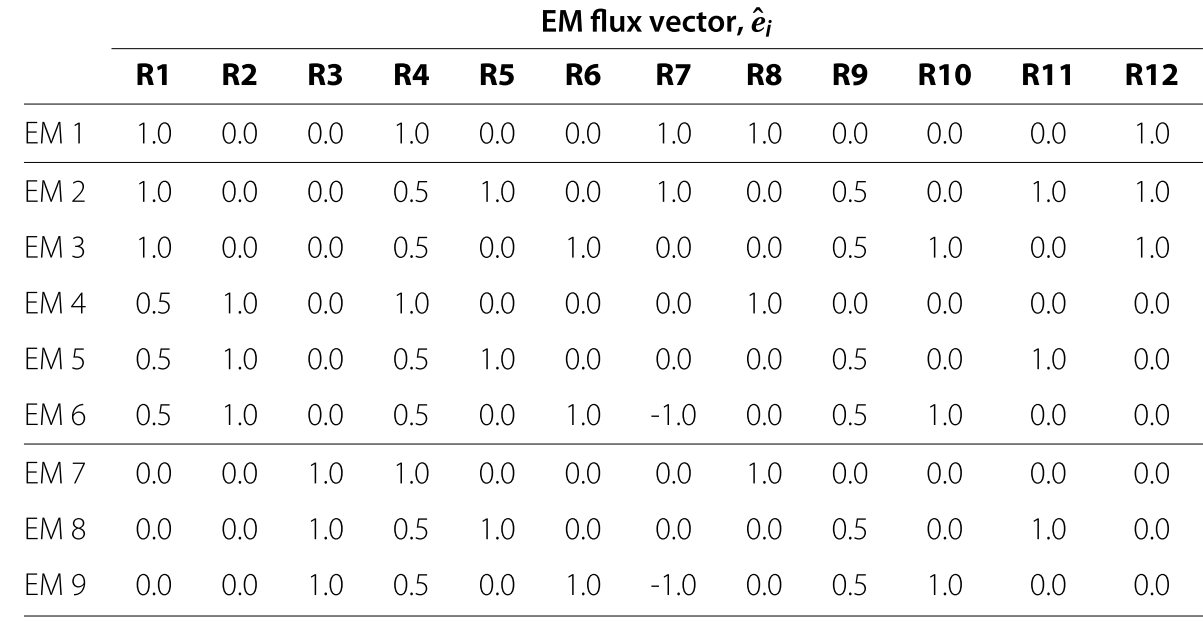
\includegraphics[width=\textwidth]{grafik/table1a} \\
\end{frame}


\begin{frame}{Binary representation of EM}
    Given an elementary mode $m \in C$ its binary representation is $e = e(m)$ where
    $$
        e_{i} := % e(m_{i})) = 
        \begin{cases}
            1 & \text{if }  m_{i} \neq 0 \\
            0 & \text{if }  m_{i} = 0 
        \end{cases}
    $$
%    $ e^{T}v \leq e^{T}e = \sum_{i=1}^{n} e_{i}^{2} = \sum_{i=1}^{n} e_{i} =: \|e\|$
\end{frame}


\begin{frame}{Group elementary modes}
    Given all $q$ elementary modes of a metabolic network.
    Group them in three sets:
    \begin{align*}
        & (e_{1}, ..., e_{r})            &\text{\emph{goal set} with desirable EM}   &\\
        & (e_{r+1}, ..., e_{r+s})        &\text{\emph{kill set} with unwanted EM}      &\\
        & (e_{r+s+1}, ..., e_{r+s+t})    &\text{\emph{helper set} with tolerated EM}         &\\
    \end{align*}
where $q = r+s+t$
\end{frame}



\bibliographystyle{apalike}
\begin{frame}{List of binary EM sets}
    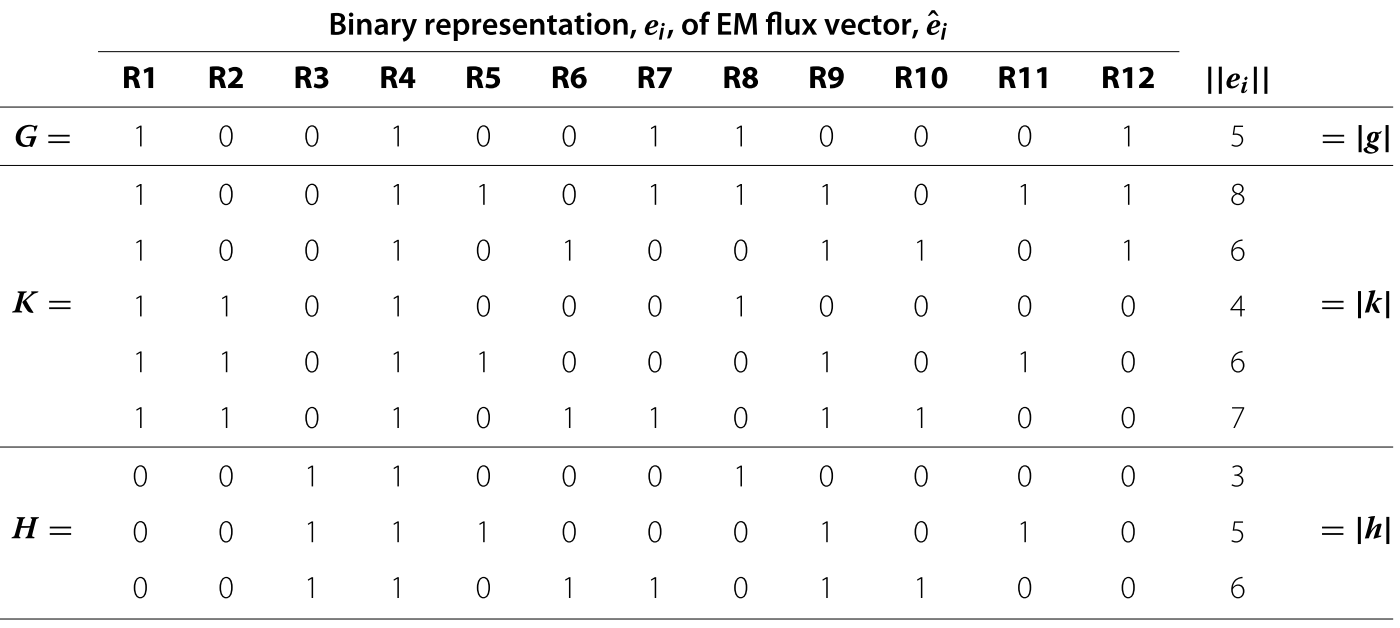
\includegraphics[width=\textwidth]{grafik/table1b}
\pause    
    \begin{block}{Problem}
        Find the minimal number of reaction \emph{knockouts} to destroy unwanted EM
        and leave goal EM
    \end{block}
\end{frame}

%%%%%%%%%%%%%%%%%%%%%%%%%%%%%%%%%%%%%%%%%%%%%%%%%%%%%%%%%%%%%%%%%%%%%%%%
\subsection{Binary linear program (BLP)}


\begin{frame}{Binary linear program (BLP)}
    
$max ~\|x\|$ \hfill $x = (x_{1}, ..., x_{n})^{T}, \quad x_{i} \in \{0, 1\} \forall i$ \\
~\\
\pause
subjected to  
\begin{align*}
    e^{T}_{g} x & =       \|e_{g}\|      & g \in \{1, ..., r\}     
    & \quad\text{\emph{(desirable EM)}}\\
    e^{T}_{k} x & \leq    \|e_{k}\|-1     & k \in \{r+1, ..., r+s\} 
    & \quad\text{\emph{(unwanted EM)}}\\
    e^{T}_{h} x & \leq    \|e_{h}\|  & h \in \{r+s+1, ..., r+s+t\}
    & \quad\text{\emph{(tolerated EM)}}\\
\end{align*}

%where
%\begin{align*}
%    |g| &= (\|e_1\|, ..., \|e_r\|)^T \\
%    |h| &= (\|e_{r+1}\|, ..., \|e_{r+s}\|)^T \\
%    |k| &= (\|e_{r+s+1}\|, ..., \|e_{r+s+t}\|)^T \\
%\end{align*}
\pause
~\\
minimal number of deletions $\Delta_{min} = n - \|x\|$

\end{frame}


\begin{frame}{BLP for example network}
\small
$$max \sum_{i=1}^{12} x_i$$
subjected to  
\begin{align*}
%\text{subject to}\quad\quad\quad\quad
    x_1 + x_4 + x_7 + x_8 + x_{12}                      & = 5   \\
    \\
    x_1 + x_4 + x_5 + x_7 + x_8 + x_9 + x_{11} + x_{12} & \leq 7 \\
    x_1 + x_4 + x_6 + x_9 + x_{10} + x_{12}             & \leq 5 \\
    x_1 + x_2 + x_4 + x_8                               & \leq 3 \\
    x_1 + x_2 + x_4 + x_5 + x_9 + x_{11}                & \leq 5 \\
    x_1 + x_2 + x_4 + x_6 + x_7 + x_9 + x_{10}          & \leq 6 \\
    \\
    x_3 + x_4 + x_8                                     & \leq 3 \\
    x_3 + x_4 + x_5 + x_9 + x_{11}                      & \leq 5 \\
    x_3 + x_4 + x_6 + x_7 + x_9 + x_{10}                & \leq 6 \\
    \end{align*}
\end{frame}

\bibliographystyle{apalike}
\begin{frame}{Find alternative solutions}
\begin{itemize}
    \item The BLP may have no or a finite number of solutions.
    \item Iteratively forbid the $j$-th solutions $x^{(j)}$ by adding constraints:
\end{itemize}
    
    \begin{align*}
        \sum_{i \in B} x_i & \leq |B| -1 & 
        \text{\emph{\textcolor{blue}{"no-good cut"}}}\\
        \sum_{i \in N} x_i & \geq 1   & ~\\
    \end{align*}
    where 
    \begin{align*}
        B = \{i |x_{i}^{(j)} = 1\} \\
        N = \{i |x_{i}^{(j)} = 0\} \\
    \end{align*}

\end{frame}


\begin{frame}{Minimal cut sets}
    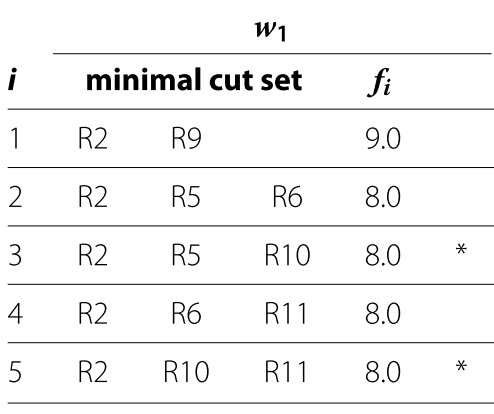
\includegraphics[height=5cm]{grafik/table2a} \\
\end{frame}

%%%%%%%%%%%%%%%%%%%%%%%%%%%%%%%%%%%%%%%%%%%%%%%%%%%%%%%%%%%%%%%%%%%%%%%%
\subsection{Biological feasibility}

\begin{frame}{Biological feasibility}
    Problem:
    \begin{itemize}
        \item Gene-enzyme-reaction mapping not always known
        \item Distinguish chemical from genetic interventions
    \end{itemize}
\pause
    Solution: 
    \begin{itemize}
        \item Add weights to objective function
        $$max \|w^T x\| $$
        \item Low weights for uptake reactions
        \item High weights for reactions with missing genetic information
    \end{itemize}
    \begin{example}
        $$w_2^T = (0.1, ~ 0.1, ~ 0.1, ~ 99, ~ 1, ~ 99, ~ 2, ~ 1, ~ 99, ~ 1, ~ 1, ~ 99)$$
    \end{example}
\end{frame}\bibliographystyle{apalike}

\begin{frame}{Minimal cut sets with weight-function}
    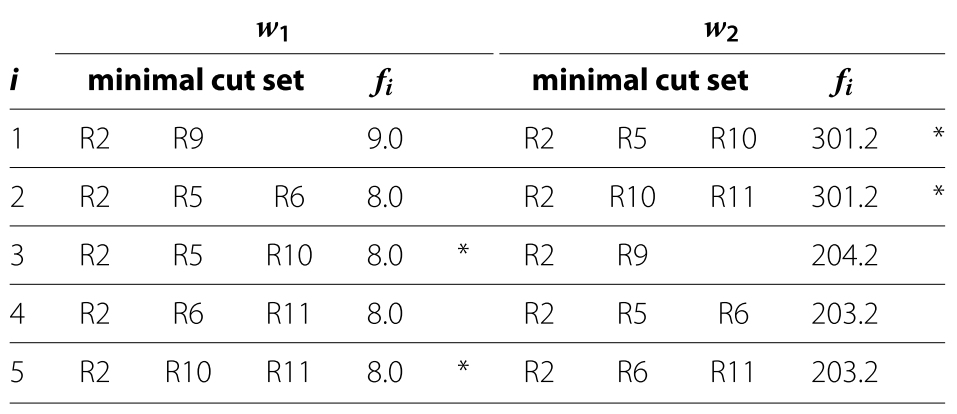
\includegraphics[height=5cm]{grafik/table2} \\
\end{frame}

%%%%%%%%%%%%%%%%%%%%%%%%%%%%%%%%%%%%%%%%%%%%%%%%%%%%%%%%%%%%%%%%%%%%%%%%
\subsection{Including regulation}
\begin{frame}{Including regulation in example}
    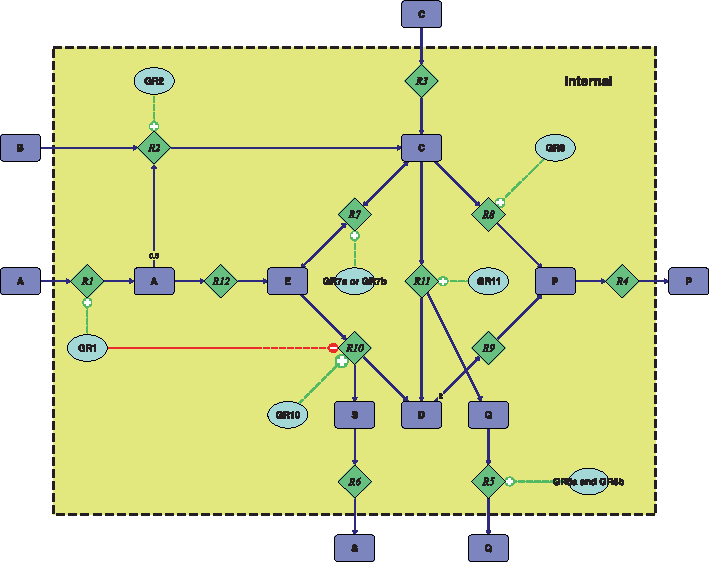
\includegraphics[width=.9\textwidth]{grafik/fig1} \\
\end{frame}


\begin{frame}{Including regulation}
\begin{itemize}
    \item Regulatory information can be modelled by Boolean functions.
    \item Each gene $g$ is represented by a logical variable $y_{g} \in \{0,1\}$.
    \item Boolean functions can be converted to inequalities.
    \item New objective function 
    $$max \quad \|w_{2}^{T} x \| + \|y\| $$
    \begin{example}
        $$ y =  (y_{1} \quad y_{2} \quad y_{5a} \quad y_{5b} \quad y_{7a} \quad y_{7b} \quad y_{8} \quad y_{10} \quad y_{11})$$
    \end{example}
\end{itemize}

\end{frame}

\begin{frame}{Convert Boolean functions to BLP constraints}
\begin{tabular}{|P{4cm} | c |r |}
\hline
Regulation type  &  Boolean function     &  BLP constraint \\
\hline
\hline
single enzyme 
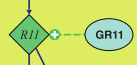
\includegraphics[height=1cm]{grafik/catalyse}
  & $G  	\mapsto R$    & $G -R = 0$ \\ 
\hline
 inhibition

\includegraphics[height=1cm]{grafik/inhibition}    
 & $\neg G \mapsto R$ & $G + R = 1 $ \\
\hline
enzyme complex   
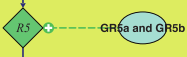
\includegraphics[height=1cm]{grafik/complex}
 & $G_{a} \land G_{b} \mapsto R $ &  $0 \leq G_{a} + G_{b} - 2R \leq 1 $\\
\hline
isoenzyme \newline 
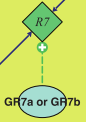
\includegraphics[height=2cm]{grafik/isoenzyme}
 &   $G_{a} \lor G_{b} \mapsto R$  &   $-1 \leq G_{a} + G_{b} - 2R \leq 0 $ \\
\hline
\end{tabular}

\end{frame}

\begin{frame}{Extendable to more complex expressions}
    \centering
    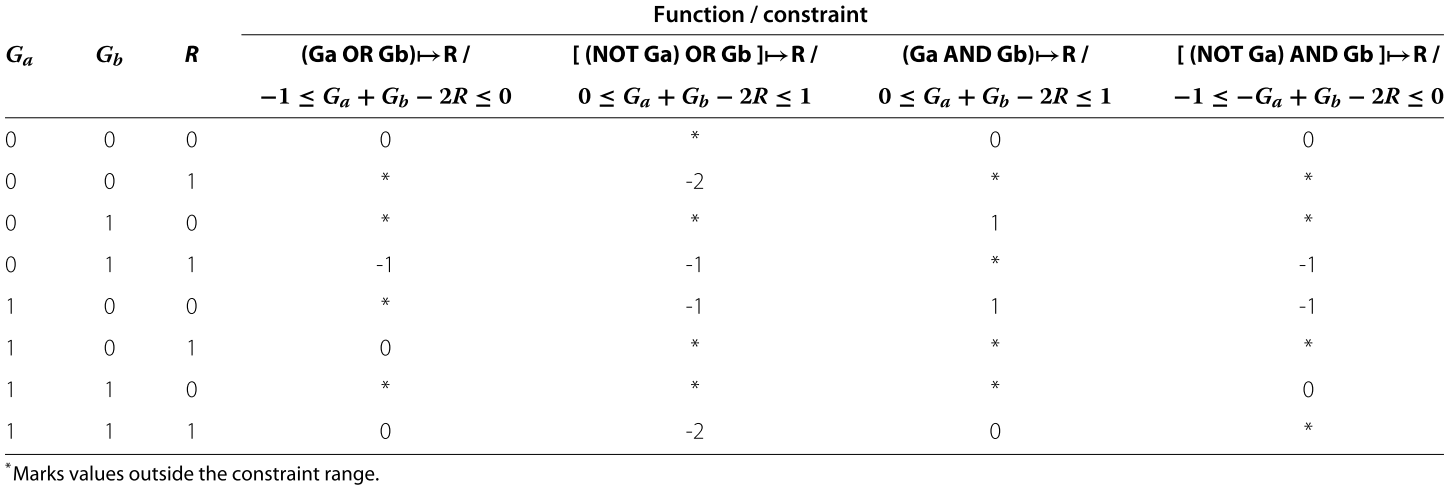
\includegraphics[width=1\textwidth]{grafik/table3}
\end{frame}

\begin{frame}{Adding regulatory constraints to the example}
    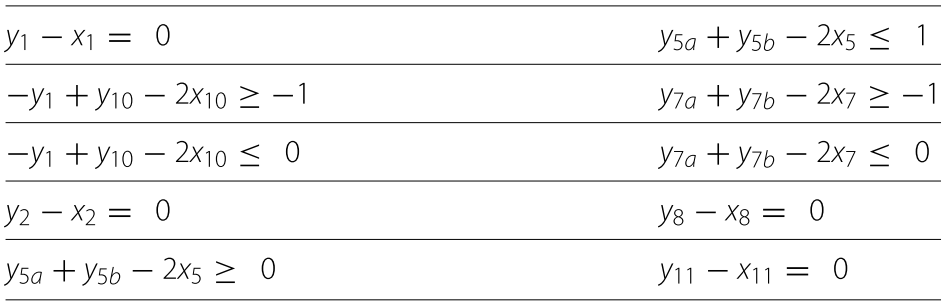
\includegraphics[width=1\textwidth]{grafik/table4} \\
\end{frame}

\begin{frame}{Minimal cut sets with weight-function and regulation}
    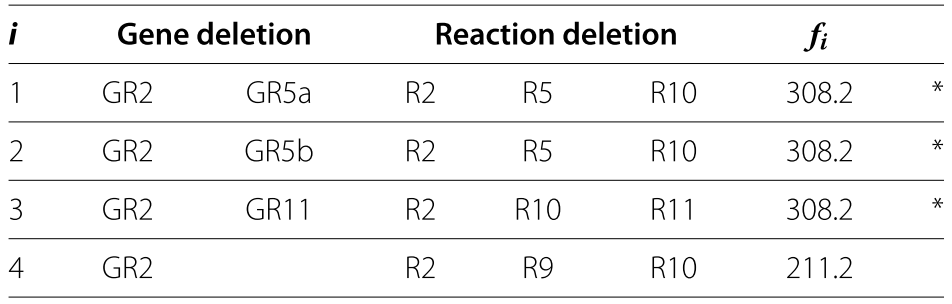
\includegraphics[width=1\textwidth]{grafik/table5}    
\end{frame}

%%%%%%%%%%%%%%%%%%%%%%%%%%%%%%%%%%%%%%%%%%%%%%%%%%%%%%%%%%%%%%%%%%%%%%%% 
\section{Results of realistic example}
%%%%%%%%%%%%%%%%%%%%%%%%%%%%%%%%%%%%%%%%%%%%%%%%%%%%%%%%%%%%%%%%%%%%%%%% 
\subsection{Ethanol production in E. coli}
%%%%%%%%%%%%%%%%%%%%%%%%%%%%%%%%%%%%%%%%%%%%%%%%%%%%%%%%%%%%%%%%%%%%%%%% 
\begin{frame}{Realistic example: Ethanol production in E. coli}
	\begin{itemize}
		\item Efficient production of ethanol from glucose in \emph{E.coli}
		\item Small scale metabolic network under anaerobic conditions
		\begin{itemize}
			\item 5,010 EM given
			\item 12 EM contribute to the optimal design
			%\item Network of minimal functionality known with seven knock-outs
		\end{itemize}
\pause
	\begin{block}{Problem}
		 Find optimal strain design with minimal number of knockouts.
	\end{block}
\pause
		\item BLP model:
		\begin{itemize}
			\item \emph{goal} set contains the 12 optimal EM
			\item \emph{kill} set contains all remaining 4,998 EM
			\item \emph{help} set is $\emptyset$
		\end{itemize}
	\end{itemize}
\end{frame}

\begin{frame}{Results: Ethanol production in E. coli}
	\begin{itemize}
	\item Results in 1,048 MCS of which 252 had only 7 deletions.
	\item 71\% are not deletable due to missing annotations.
	\end{itemize}
~\\
\pause
With weight function (models biological feasibility):
	\begin{itemize}
		\item 8 alternative MCS with 7 feasible gene deletions		
	\end{itemize}
~\\
$\Rightarrow$ Outperforms an  experimentally implemented strain with 8 knockouts.
\end{frame}

\begin{frame}{Realistic example: Full model}
    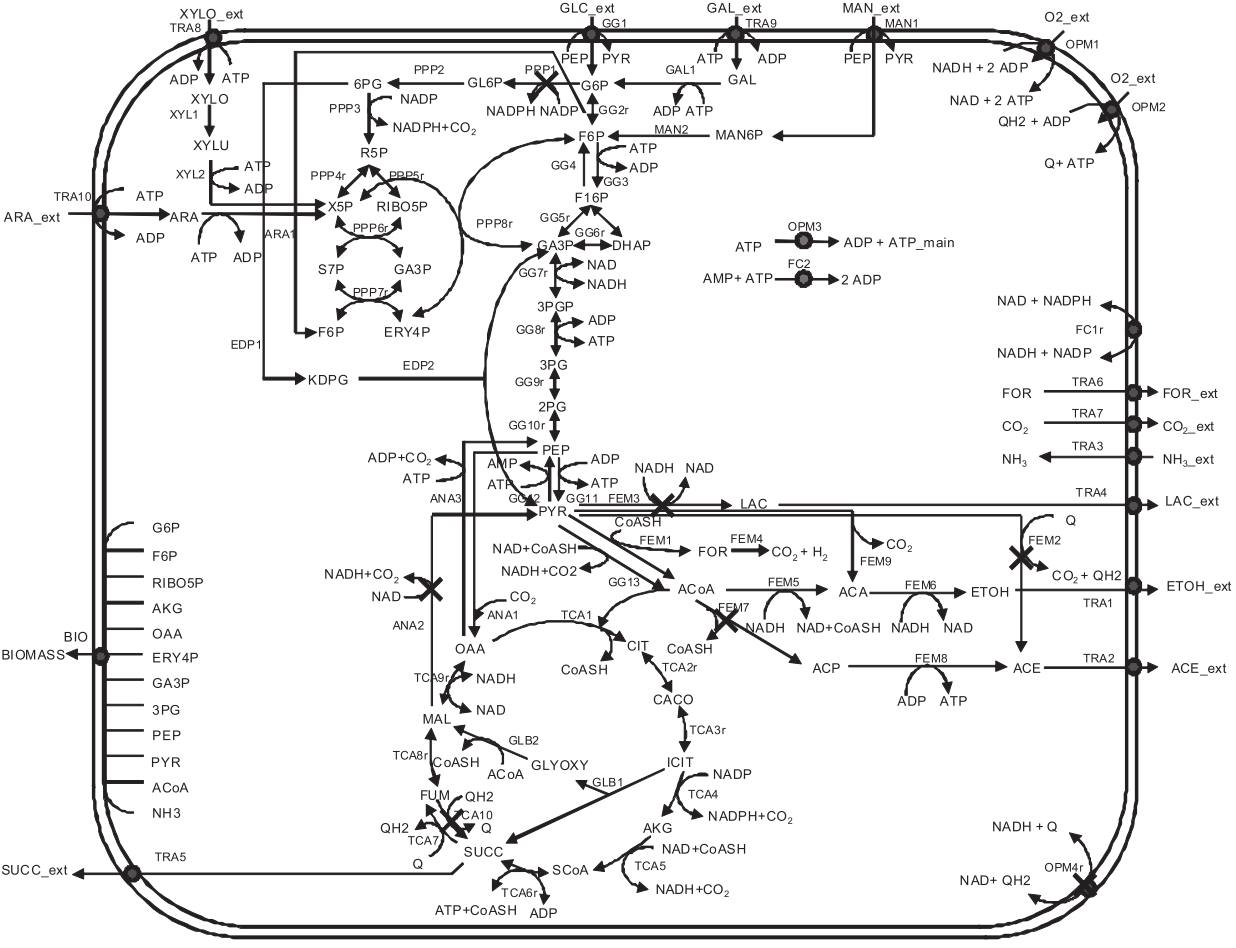
\includegraphics[height=.86\textheight]{grafik/fullmodel} \\
    \tiny{source: Trinh et al. (2008) Applied and environmental microbiology}
\end{frame}

\begin{frame}{Realistic example: Full model}
Repeat analysis with full \emph{E.coli} model 
(without restriction to glucose uptake under unaerobic conditions)
\pause
\begin{itemize}
	\item 429,276 EM (disregarding two substrate cycles) %futile cycle)
	\item $\Rightarrow$ 55,488 MCS (1,440 with minmal number of 11 reaction deletions)
	\item $\Rightarrow$ 27\% of all and none of optimal MCS are fully annotated
\pause
	\item With weight function:
	\begin{itemize}
		\item 12 reaction deletions
		\item 5 out of the 12 are uptake reactions
	\end{itemize}
\end{itemize}
$\Rightarrow$ Recovers the original model with anaerobic growth on glucose

\end{frame}

%%%%%%%%%%%%%%%%%%%%%%%%%%%%%%%%%%%%%%%%%%%%%%%%%%%%%%%%%%%%%%%%%%%%%%%%
\subsection{Complexity and runtime}

\begin{frame}{Complexity and runtime}
\begin{itemize}
	\item BLP is a special case of integer liner programming (ILP) which is NP-complete. 
	\item Number of EM explodes combinatorially with system size \\
	 $\Rightarrow$ EM analysis is restricted to 
	small scale networks with hundreds of reactions/variables.
\pause	
    \item Efficient ILP solvers are available. 
    \item Compress redundant constraints in preprocessing step 
	\begin{itemize}
		\item Full \emph{E.coli} model: 420,276 constraints for 71 variables
		\item Transformed into 28 constraints for 34 variables
	\end{itemize}
	\item Method is still scalable: \\
	It finds all 2.304 MCS in model with 271 million EM in 122 seconds. 
\end{itemize}
$\Rightarrow$ The problem is the calculation of all EM in the first place.
\end{frame}

%\begin{frame}{Limitations}
%	\begin{itemize}
%		\item Some regulatory information like Feedback-Loops can not be modeled
%	\end{itemize}
%\end{frame}
\begin{frame}{Limitations}
\begin{itemize}
    \item Elementary modes have to be computed first (\emph{efmtool}).
    \item Optimal and unwanted EM have to be known.
    \item Not all EM are considered. Unnecessary constraint definitions for tolerated EM. 
%    \item Substrate cycles can not be modelled.
    \item Only explicit Boolean functions can be modelled, \\
    e.g. $G \textcolor{green}{\mapsto} R \leadsto G -R = 0$
    which is equivalent to  $G  \textcolor{red}{\iff} R$.
    \item Negative feedback loops cause infeasibility. \\
        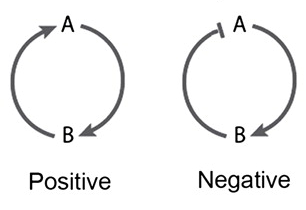
\includegraphics[width=0.3\textwidth]{grafik/feedbackloop} \\
        \tiny{source: Herranz et al. (2010) Genes \& development} \\
        \normalsize
\begin{align*}
    A \mapsto B        & \quad \leadsto \quad A \iff B       & \quad \leadsto \quad A - B = 0 \\
    B \mapsto \neg A   &  \quad \leadsto \quad  B \iff \neg A & \quad \leadsto \quad A + B = 1  \\
\end{align*}

\end{itemize}
\end{frame}



%%%%%%%%%%%%%%%%%%%%%%%%%%%%%%%%%%%%%%%%%%%%%%%%%%%%%%%%%%%%%%%%%%%%%%%% 
\section{Summary and conclusions}
%%%%%%%%%%%%%%%%%%%%%%%%%%%%%%%%%%%%%%%%%%%%%%%%%%%%%%%%%%%%%%%%%%%%%%%% 
\begin{frame}{Summary and conclusion}
\begin{itemize}
    \item Elementary flux modes represent biological pathways 
        in metabolic networks under the steady state assumption.
    \pause
    \item A minimal cut set (MCS) of reaction knockouts is needed to optimize 
    metabolic engineering like glucose production in bacterial strains.
    \pause
    \item A simple integer linear program predicts minimal intervention strategies.
    \pause
    \item A weight function account for experimental difficulties in implementing a reaction deletion \emph{in vivo}.
    \pause
    \item Regulatory information and gene-enzyme-reaction mapping 
    can be included by additional variables and constraints.
    \pause
    \item The evaluation on real data results in an improved design  
    of an implemented \emph{E.coli} strain.
\end{itemize}	
\pause
\begin{block}{Conclusion}
    Binary linear programming is a simple and flexible method for 
    elementary flux mode analysis and strain design.
\end{block}
\end{frame}

\begin{frame}
\begin{center}    
    \nocite{Jungreuthmayer2012}
    \large Thank you!
\end{center}
 ~ \\
 ~ \\
\normalsize
Reference: \\
\bibliography{uni}

\end{frame}

\end{document}
%%%%%%%%%%%%%%%%%%%%%%%%%%%%%%%%%%%%%%%%%%%%%%%%%%%%%%%%%%%%%%%%%%%%%%%% 
% Stuff:
%%%%%%%%%%%%%%%%%%%%%%%%%%%%%%%%%%%%%%%%%%%%%%%%%%%%%%%%%%%%%%%%%%%%%%%% 

%TODO:
%   # irreversable reactions in model
%   # constraints for binary variables in IP 
%	# use colors
%   # MCS definition
%	# NMF def.
%	# Finds all solutions
%   # Limitations (in context?)
%   # xout H constraints
%   - check second constraints by iteratrion
%   # sources / other papaers
